\documentclass{article}
\usepackage{geometry}
\usepackage{minted}
\usepackage{amsmath}
\usepackage{float}
\usepackage{graphicx}

\geometry{a4paper, left=1in, right=1in, top=1in, bottom=1in}

\title{ECEN 759 Lab 7: Differential Fault Analysis Attack on AES}
\author{S M Farabi Mahmud}


\begin{document}
\maketitle
\section{Preliminaries on AES}
Since we are using a AES with 128 bit key length, there are 10 rounds of operation in total. First 9 rounds consists of the following operations - 
\begin{itemize}
	\item Shift Rows \textbf{SR}
	\item Sub Byte \textbf{SB}
	\item Mix Column \textbf{MC}
	\item Add Round Key \textbf{RK}
\end{itemize}
However, in the last round, we do not have the \textbf{MC} operation. 
We express the key of each i-th round as $K^i$ The plaintext and the ciphertext is denoted by $P$ and $C$ respectively. $M^i_j$ denotes the j-th byte at i-th round. 

\section{Reverse Key Scheduling}
We know the key scheduling algorithm uses specific algorithm to generate all the round keys from the master key. We use the exact inverse order to generate the round keys from the later round keys. For this purpose, we use the following code - 
\begin{listing}[H]
	\begin{minted}[linenos]{python}
def gfunction(w,round_constant):
  return [sbox[w[1]] ^ round_constant,sbox[w[2]],sbox[w[3]],sbox[w[0]]]
	
def prev_roundkey(arr, round_constant):
  prev_arr = []
  w4 = [arr[0],arr[1],arr[2],arr[3]]
  w5 = [arr[4],arr[5],arr[6],arr[7]]
  w6 = [arr[8],arr[9],arr[10],arr[11]]
  w7 = [arr[12],arr[13],arr[14],arr[15]]

  w3 = [x^y for x,y in zip(w6,w7)]
  gw3 = gfunction(w3, round_constant)
  w2 = [x^y for x,y in zip(w5,w6)] 
  w1 = [x^y for x,y in zip(w4,w5)]
  w0 = [x^y for x,y in zip(w4,gw3)]
  prev_arr.extend(w0)
  prev_arr.extend(w1)
  prev_arr.extend(w2)
  prev_arr.extend(w3)

  return prev_arr

	\end{minted}
\end{listing}

\section{Single Bit Fault Attack}
In this section, we will describe how we have implemented the single bit fault attack on AES. We used the concept from Giraud's work~\cite{giraud2004dfa}. In the first attack, we target the one bit of the input of the Round 10 that is denoted by $M^9$.
\begin{listing}[H]
\begin{minted}[linenos]{python}
def dfa_bit_fault(c, ds):
  locations = [0x1, 0x2, 0x4, 0x8, 0x10, 0x20, 0x40, 0x80]
  recovered = []
  for j in range(16):
    count = [0]*255
    for x in range(255):
        for e in locations:
            for d in ds:
                lhs = c[0][shift_row_index(j)] ^ d[shift_row_index(j)]
                rhs = subbyte(x) ^ subbyte(x ^ e)
                if (lhs == rhs):
                    count[x] = count[x]+1
    recovered.append(np.argmax(count))
  return recovered    
\end{minted}
	\caption{Main loop for the DFA Single Bit Fault Attack}
	\label{single-bit-fault}
\end{listing}

For this reason, we can directly determine that the output of Round 10, the ciphertext C that follows the equation - 
\begin{equation}
C_{SR(j)} = SB(M^9_j) \oplus K^{10}_{SR(j)}
\label{normalc}
\end{equation}


Here, in this equation~\ref{normalc}, we can get the output of the round 10, the ciphertext C from the input of the Round 10 $M^9$ and the XORing that with the round key $K^{10}$. If we apply a fault $e_j$ on one bit of the $j$-th byte of the $M^9$ we can get the faulty ciphertext $D$ following the equation \ref{faultyD}

\begin{equation}
	D_{SR(j)} = SB(M^9_j \oplus e_j) \oplus K^{10}_{SR(j)}\label{faultyD}
\end{equation}

XORing equation \ref{normalc} and equation \ref{faultyD} we can get - 
\begin{equation}
C_{SR(j)}  \oplus	D_{SR(j)} = SB(M^9_j)   \oplus SB(M^9_j \oplus e_j)   \label{xor_c_d}
\end{equation}
We have only one bit fault, so possible location $e_j \in \{0x01, 0x02, 0x04,0x08,0x10,0x20,0x40,0x80\}$. Again, one bit fault at $M^9$ impacts only one byte of the faulty ciphertext $D$, we can generate all possible values for the $M^9$ in range $\{0,1,\ldots, 255\}$ and all possible bit locations and see if the equation~\ref{xor_c_d} holds for these values. Then we determine the possible value of the recovered key from the maximum of the count. 

\subsection{Results}
After running the code, first we get the round key for the 10th Round. From there using the Reverse Key Scheduling algorithm, we get the following results - 

\begin{table}[H]
	\begin{tabular}{|c|c|}
		\hline 
		\textbf{Round} & \textbf{Round Key} \\ \hline 

10 & dfb15c7948b0a6f353222dec717e0ce7 \\ \hline
9 & a34c77ea9701fa8a1b928b1f225c210b \\ \hline
8 & 33e08df8344d8d608c93719539ceaa14 \\ \hline
7 & ff59812d07ad0098b8defcf5b55ddb81 \\ \hline
6 & 539513faf8f481b5bf73fc6d0d832774 \\ \hline
5 & ff2cc7cdab61924f47877dd8b2f0db19 \\ \hline
4 & 1a08bf2b544d5582ece6ef97f577a6c1 \\ \hline
3 & 93330eff4e45eaa9b8abba1519914956 \\ \hline
2 & 173e14cddd76e456f6ee50bca13af343 \\ \hline
1 & 5d340296ca48f09b2b98b4ea57d4a3ff \\ \hline \hline 
\textbf{Master Key} & 75c45b86977cf20de1d044717c4c1715 \\ \hline
	\end{tabular}
\end{table}

\section{Byte Fault Attack}
In this section we have followed the attack suggested in the paper by Michael Tunstall et al~\cite{tunstall2011differential}. Since this attack induces faults at one of the 4 bytes of the top row of input to the eighth round, $M^8$. Since we will have two rounds of SR, SB and RK and one round of MC on this $M^8$ we can use to solve the following set of equations~\ref{setofeq} to determine the possible values of key at Round 10 from the ciphertext c. Here $SB^{-1}$ denotes the inverse of Shift Byte operations. $x_i$ denotes the i-th byte of the correct ciphertext and $x^\prime_i$ denotes the i-th byte of the faulty ciphertext. $k_i$ denotes the i-th byte of the Round 10 roundkey. $f$ denotes the faulty byte location. 
\begin{equation}
\begin{aligned}
2f &= SB^{-1}(x_0 \oplus k_0) \oplus SB^{-1}(x^\prime_0 \oplus k_0)\\
2f &= SB^{-1}(x_1 \oplus k_1) \oplus SB^{-1}(x^\prime_1 \oplus k_1)\\
2f &= SB^{-1}(x_2 \oplus k_2) \oplus SB^{-1}(x^\prime_2 \oplus k_2)\\
2f &= SB^{-1}(x_3 \oplus k_3) \oplus SB^{-1}(x^\prime_3 \oplus k_3)\\
3f &= SB^{-1}(x_4 \oplus k_4) \oplus SB^{-1}(x^\prime_4 \oplus k_4)\\
3f &= SB^{-1}(x_5 \oplus k_5) \oplus SB^{-1}(x^\prime_5 \oplus k_5)\\
3f &= SB^{-1}(x_6 \oplus k_6) \oplus SB^{-1}(x^\prime_6 \oplus k_6)\\
3f &= SB^{-1}(x_7 \oplus k_7) \oplus SB^{-1}(x^\prime_7 \oplus k_7)\\
f &= SB^{-1}(x_8 \oplus k_8) \oplus SB^{-1}(x^\prime_8 \oplus k_8)\\
f &= SB^{-1}(x_9 \oplus k_9) \oplus SB^{-1}(x^\prime_9 \oplus k_9)\\
f &= SB^{-1}(x_{10} \oplus k_{10}) \oplus SB^{-1}(x^\prime_{10} \oplus k_{10})\\
f &= SB^{-1}(x_{11} \oplus k_{11}) \oplus SB^{-1}(x^\prime_{11} \oplus k_{11})\\
f &= SB^{-1}(x_{12} \oplus k_{12}) \oplus SB^{-1}(x^\prime_{12} \oplus k_{12})\\
f &= SB^{-1}(x_{14} \oplus k_{14}) \oplus SB^{-1}(x^\prime_{14} \oplus k_{14})\\
f &= SB^{-1}(x_{13 }\oplus k_{13}) \oplus SB^{-1}(x^\prime_{13} \oplus k_{13})\\
f &= SB^{-1}(x_{15} \oplus k_{15}) \oplus SB^{-1}(x^\prime_{15} \oplus k_{15})\label{setofeq}
\end{aligned} 
\end{equation}

We iterate through all possible values of $f, k_i \in \{0,1,\dots,255\}$ to determine for which value the equations of the systems of equations~\ref{setofeq} is valid. Here for each faulty byte, we have to satisfy four equations containing four locations of the key. We can get that from the following figure~\ref{fig:task2}. For example, byte 0 impacts the $k_0, k_7, k_{10}, k_{13}$. So we do not need to check beyond the equations related with these locations. 

\begin{figure}[H]
	\centering
	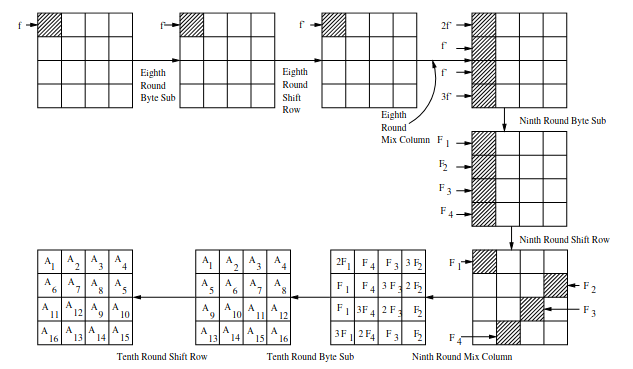
\includegraphics[width=\linewidth]{task2}
	\caption{Change in one byte impacting 4 bytes in Round 10}
	\label{fig:task2}
\end{figure}

To determine the round key of 10th Round, we have used the following code given at Listing~\ref{codetask2}. We have used the counting method to determine the values that appear for most of the time for the solutions that have solved the equations~\ref{setofeq}

\begin{listing}[H]
\inputminted[linenos,tabsize=2,breaklines]{python}{task2.py}\label{codetask2}
\end{listing}


\subsection{Results}
After running the code, first we get the round key for the 10th Round. From there using the Reverse Key Scheduling algorithm, we get the following results - 

\begin{table}[H]
	\begin{tabular}{|c|c|}
		\hline 
		\textbf{Round} & \textbf{Round Key} \\ \hline 
10 & 21a689161102fd820e0336150022956e \\ \hline
9 & eaaca8bd30a474941f01cb970e21a37b \\ \hline
8 & 46e9663fda08dc292fa5bf03112068ec \\ \hline
7 & 51e7b98d9ce1ba16f5ad632a3e85d7ef \\ \hline
6 & 256a1f92cd06039b694cd93ccb28b4c5 \\ \hline
5 & 465686a8e86c1c09a44adaa7a2646df9 \\ \hline
4 & 67ffdec7ae3a9aa14c26c6ae062eb75e \\ \hline
3 & 5f5c5211c9c54466e21c5c0f4a0871f0 \\ \hline
2 & a18444d3969916772bd91869a8142dff \\ \hline 
1 & 1e12d43f371d52a4bd400e1e83cd3596 \\ \hline \hline 
\textbf{Master Key} & 42f0108d290f869b8a5d5cba3e8d3b88 \\ \hline
	\end{tabular}
\end{table}

\subsection{GitHub}
\bibliographystyle{acm}
\bibliography{refs.bib}
\end{document}